%% Copyright 2022 Zijian Wang. All rights reserved.
%% Email: felix_wzj@yahoo.com
%% The newest version can be obtained from GitHub.

\documentclass{article}

\usepackage{amsmath, amssymb, graphics, setspace}
\usepackage[letterpaper, total={6.5in, 9in}]{geometry}
\usepackage{cite}
\usepackage{tikz}
\usepackage{tikz-cd}
\usepackage{float, multicol}
\usetikzlibrary{positioning, cd}

\newcommand{\mathsym}[1]{{}}
\newcommand{\unicode}[1]{{}}

\setlength{\parskip}{0.8em}

\begin{document}

\title{A new type of automated prover based on category theory}
\author{Zijian Wang}
\date{}
\maketitle

\begin{center}
Northern Eastern Yucai School, Shenyang, Liaoning, P.R.China
\end{center}

\hrule
\begin{abstract}
In this article I present a new type of automated statement proof algorithm based on new data structures, i.e. brackets and map graphs
and new algorithms. The brackets provide an elegant low-knowledge representation of mathematical concepts. The map graphs offer an efficient machine-learning method which let the computer learn knowledge while proving. Additionally, the new finding is totally built on the category theory. Furthermore, a prototype of the program is given.
\end{abstract}
\hrule

\section*{Introduction}
During the long period of development of the research on automated theorem provers, there have already existed a great number of research and implementation on proofs focusing on a specific mathematical subject, such as algebra equations (for example, Wolfram Mathematica{'}s FindEquationProof function \cite{2}) or geometrical theorems (for example, the Geometry Expert or GEX \cite{3} of Key Laboratory of Mathematics Mechanization, Chinese Academy of Sciences). Some relatively new works in this aspect includes Microsoft{'}s Lean prover and Z3 algorithm.

However, if we investigate deeper into these algorithms, we will find the fact that all of these provers stand on the basis of logic theories. Both completely automated theorem provers and semi-automated computer auxiliary statement provers like Coq and Isabelle, are designed to follow certain logic rules and generate results as logic formulas. Nevertheless, although we have to admit that such do is an effective method, this method also sets an insurmountable limit on the execution that the program could not think comprehensively such as solving an algebra problem in a geometrical way.

When we humans think of mathematical problems and perform proofs, we do not follow purely logical ways like complex stuff like Cooper{'}s algorithm. Instead, we just perform tries to seek breakthrough points using his knowledge in a diversified thought. Why cannot programs do things like that? Why can not they perform some sort of knowledge transferring? Carry this question and in experimental and curious attitude, I conducted the research on this topic and have found a utility to do the task: the category theory.

Mainly developed in the twentieth century by the contribution of MacLane and Eilenberg with the purpose to investigate algebra topology, the category theory is a fast-evolving aspect of modern mathematics. In just a few decades, the category theory has become the standard and formal language of homology algebra and algebraic geometry and has gained a lot of meaningful achievements, for instance the Yoneda{'}s Lemma and Braid categories, which serves as a neat explanation for the Yang-Baxter Equation (YBE). Moreover, the category theory{'}s main idea, which is to put mathematical structures into categories satisfies the worldview of the Bourbaki school.

In this paper I will present a new approach of automated proving using knowledge of the category, as well as its theoretical foundation, and will provide a new algorithm which can prove mathematical statements comprehensively. Additionally, an executable program and its implementation process will be describe later.

\textit{ Structure of the paper.}\\
The paper mainly consists of seven sections. The Introduction section demonstrates the background of the research and fundamental opinions around it. The Preliminaries section, made up of two subsections, claims to minimized pre-knowledge required to understand the paper and the symbols I select to use. The third section defines a set of mathematical structures that will be used by the algorithm. The forth section explains the detailed workflow procedures of the algorithm. The next section claims the conclusions of the research and the to-do improvements in the future. Finally the Acknowledgments section expresses my gratitude to the help and the References section claims the referential resources used while conducting the project.f

\section*{Preliminaries}

\subsection*{Notations and Conventions}

To begin with, we use notation \(\mathcal{C}\) to demonstrate a category and use script\(\mathcal{F}\) to present a functor. \(\mathcal{U}\) stands for the Grothendieck universe selected and \(\mathcal{F}\mathit{o}\mathit{r}\) stands for the forgetful functor. A map is noted in one of the two following forms:

\[f: A\to B\]
\[x\mapsto y\]

where \(A\) and \(B\) are sets and\(x\)and \(y\) are elements in \(A\) and \(B\).

 Furthermore, we use \(s(f)\) for the source object of morphism \(f\)\textit{  }and use \(t(f)\) for the target object of morphism\(f\). The symbol \(\text{Ob}(\mathcal{C})\) stands for the object collection for the category \(\mathcal{C}\). We annotate the morphism set for a category with notation \(\text{Mor}\) and annotate the \(\text{Hom}-\text{set}\) for a category \(\mathcal{C}\) between elements \(a\) and \(b\) with notation \(\text{Hom}_{\mathcal{C}}(a,b)\).

Basic logical operators like \(\forall\), \(\exists\) and \(\neg\) are used while basic set operators such as \(\in\), \(\subset\) and \(\cup\) are used too. In addition, we use notation \(|S|\) for the size for set \(S\).

For each ordered pair \(t=(x,y)\), we use \(t_{\ell }\) for \(x\) and \(t_{\mathit{r}}\) for \(y\).

To avoid misunderstandings, \pmb{the Zermelo-Fraenkel set theory} or ZFC as short is utilized to be the set system, with Grothendieck universe concepts added. \cite{1}

\subsection*{Pre-Knowledge}

Readers should have basic understandings of the category theory \cite{1} and axiomatic set theory. At least, they should know the basic concepts as well as these conclusions and theorems:

\pmb{ Axiom.} The Selection Axiom.

Let \(X\) be a set and each of \(X\){'}s elements not empty, then there exists function \(g:X\to \cup X\) making \(\forall x\in X,g(x)\in x\), naming \(g(x)\) as the selection function.

The selection axiom is the ninth axiom in the Zermelo-Fraenkel set system and it is equivalent to the theorem below.

\pmb{ Theorem. }The Zermelo{'}s Well-Ordering Theorem.\cite{1}

Every set \(S\) can be well-ordering as long as it has a choice function.

\pmb{ Proof:} First, we select element \(\mho \notin S\). As the ZFC system{'}s selection axiom enables to select element \(g(S')\) from each subset \(S'\) of \(S\). Let \(a_0\text{:=}g(S)\). Using transfinite recursive theorem to each ordinal \(\alpha\) we define:

\[a_{\alpha }\text{:=}\left\{
\begin{array}{cc}
 g\left(S\backslash \left\{\left.a_{\beta }\right|\beta <\alpha \right\}\right), & S\neq \left\{\left.a_{\beta }\right|\beta <\alpha \right\} \\
 \mho , & S=\left\{\left.a_{\beta }\right|\beta <\alpha \right\} \\
\end{array}
\right.\]

Then, since \(S\) is a set, a minimized \(\theta\) can be chosen making \(a_{\theta }=\mho , S=\left\{\left.a_{\beta }\right|\beta <\theta \right\}\) and significantly there exists a bijection between \(S\) and \(\theta =\{\beta |\beta <\theta \}\). Following the definition, there obviously exists a well-ordering on \(S\).
\begin{flushright}
	$\blacksquare $
\end{flushright}

Some preliminary knowledge also includes the Ebbinghaus Forgetting Curve equation \cite{4} used in this paper later. This approximate function is defined below:

\[B=\frac{100 k}{(\ln  t)^c+k}\]

Where \(B\) is percent of memorization while\(t\)is time and \(c=1.25,k=1.84\). This curve is used by the algorithm for self-optimization purposes.

So as to avoid utilization of impure functions, a pseudo random generator is used. We select the linear congruential generators \cite{5}, whose recursive equation is,

\[X_{n+1}=(\left(a X_n+c\right) \bmod M)\]

Following the ANSI C implementation, we determine the parameters used by the recursive to the followings:

\[M=2^{32},a=1103515245, c=12345\]

In this paper we use notation \(\mathit{r}\) to represent a new random number generated, which is actually a pure function of the last random number and the expression is simplified for representation{'}s explicitness.

\section*{The Computerized Representation of Mathematical Structures}

Before more specific discussion, we select Grothendieck universe \(\mathcal{U}\) \cite{1} to avoid set theory paradoxes. Besides, we define meta category \(\mathcal{C}\) where all discussions take place. There are briefly three kind of objects in \(\mathcal{C}\): symbols, notations and brackets. All symbols in \(\mathcal{C}\) forms sub category \(\text{Sym}(\mathcal{C})\) called the \pmb{ Symbol Subcategory}. All notations in \(\mathcal{C}\) forms \(\text{Not}(\mathcal{C})\) and all brackets forms \(\text{Bra}(\mathcal{C})\), called the \pmb{ Notation Subcategory} and the \pmb{ Bracket Subcategory}. That is,

\[\mathcal{C}=\text{Sym}(\mathcal{C})\sqcup \text{Not}(\mathcal{C})\sqcup \text{Bra}(\mathcal{C})\]

The three forms a partition of the big category.

Different from other implementations and research, we describe every major mathematical structure to be used in seeking for proof, from single symbols to contents of proof steps in a single data structure called brackets.

\pmb{ Definition.} A \pmb{ bracket} \(\beta\) is defined as a set of ordered pairs in the form of below:

\[\beta \text{:=}\left\{(i,x)\left|i\in \text{On}_{\geq 1}\right.,x\in \text{Sym}(\mathcal{C})\cup \text{Not}(\mathcal{C})\cup \text{Bra}(\mathcal{C})\right\}\]

\(\beta\) is valid if and only if every element of \(\beta\), its left element is unique. We define filtered subsets of \(\beta\). The \pmb{ Symbol Subset} of \(\beta _{\mathcal{S}}\text{:=}\left\{t\in \beta \left|t_{\mathit{r}}\in \text{Sym}(\mathcal{C})\right.\right\}\). Following this way, the \pmb{ Notation Subset} \(\beta _{\mathcal{N}}\) and the \pmb{ Bracket Subset} \(\beta _{\mathcal{B}}\) are defined as well. There are two types of brackets: The first type is called a \pmb{ Symbol Holder} where \(\beta =\{(i,A)\},i\in \mathbb{Z}_{\geq 1},A\in \text{Sym}(\mathcal{C})\). The second type is called a \pmb{ Compositor} where

\[\beta =\{(j,\mathcal{N})\}\cup \left\{(i,x)\left|i\in \text{On}_{\geq 1}\right., x\in \text{Sym}(\mathcal{C})\cup \text{Bra}(\mathcal{C})\right\},\forall
t\in \beta ,j\in \text{On}_{\left[1,t_{\ell }\right]}\]

Here comes an important definition about bracket isomorphism which will be referred inside the third section of this paper.

\pmb{ Definition.} Two bracket \(\alpha\) and \(\beta\), are thought to be \pmb{ isomorphic} (noted as \(\alpha \simeq \beta\)) if they satisfy the following restrictions:

First, \(|\alpha |=|\beta |\) indicating the two brackets have same cardinal numbers. Second, all right elements sorted in the order defined by the sort of the left pair elements, correspondingly, are either same or symbols with the same type. Otherwise, the two brackets are \pmb{ not isomorphic}, noted as \(\alpha \not{\simeq}\beta\).

Next we define the mathematical representation for notations. A notation is either a operator (for example, \(+\) and \(\cdot\)) or a data type (for example, number and function). Its precise declaration comes below.

\pmb{ Definition.} A \pmb{ notation} \(\mathcal{N}\) is defined as an object in \(\text{Not}(\mathcal{C})\) which is a sub category of \(\mathcal{C}\). The \(\text{Ob}(\text{Not}(\mathcal{C}))\) set can be mapped to \(\text{On}_{\geq 0}\) class, indicating the number of parameters that a notation take. In which,

\[\mathit{p}:\text{Ob}(\text{Not}(\mathcal{C}))\to \text{On}_{\geq 0}\]
\[\mathcal{N}\overset{\mathit{p}}{\mapsto }n\]

In that case if \(n=0\) then we say \(\mathcal{N}\) is a \pmb{ type} and if \(n>0\) then \(\mathcal{N}\) is an \pmb{ operator}. For instance, obviously, \(\mathit{p}(+)=2\) and \(\mathit{p}(\neg )=1\). A notation\(\mathcal{N}\) is called \pmb{ finite} if \(\mathit{p}(\mathcal{N})<\omega\), and otherwise \(\mathcal{N}\) can have infinite number of symbols as parameters, when the notation is called to be \pmb{ infinite}.

After declaring what notations are, we then define symbols. Basically, a symbol is an instance of a notation. As notations are like containers, as symbol is like the content in them. The accurate representation of a symbol comes below.

\pmb{ Definition.} A \pmb{ symbol} \(\mathcal{S}\) is defined as an object in \(\text{Sym}(\mathcal{C})\) which is a sub category of \(\mathcal{C}\). There exists a functor from \(\text{Sym}(\mathcal{C})\) to \(\text{Not}(\mathcal{C})\):

\[\nu :\text{Sym}(\mathcal{C})\to \text{Not}(\mathcal{C})\]
\[\mathcal{S}\overset{\mathit{v}}{\mapsto }\nu (\mathcal{S})\]

Where \(\nu (\mathcal{S})\) is the \pmb{ corresponding notation} of \(\mathcal{S}\) and must satisfy \(\forall \mathcal{S}\in \text{Sym}(\mathcal{C}),\mathit{p}(\nu (\mathcal{S}))=0\), indicating all corresponding notations are types instead of operators. For convenience and precision, the text that meaning creating a symbol \(\mathcal{S}\) whose corresponding notation is \(\mathcal{N}\)can and should be written in the form below.

\[\mathcal{S}\in \text{Ob}(\text{Sym}(\mathcal{C}))\land \mathit{v}(\mathcal{S})==\mathcal{N}\]

This should not be written using \(\mathcal{S}=\mathit{v}^{-1}(\mathcal{N})\) because if so, the must of \(\mathit{v}^{-1}(\mathcal{N})==\mathit{v}^{-1}(\mathcal{N})\) disables the possibility to create another instance of \(\mathcal{N}\), which is ridiculous. 

Two brackets are thought to be \pmb{ equal} when the sequences of \(t_{\mathit{r}}\), sorted via the ordering of \(t_{\ell }\) are the same and this relationship constructs a equivalence morphism between the two in the \(\text{Bra}(\mathcal{C})\) category, noted as below:

\[\epsilon :\alpha \equiv \beta\]

A bracket, in order to enhance simplicity, can be wrapped into a symbol. Therefore with these three definitions, how do we actually represent mathematical stuff? One example is how to utilize them to express one of the most basic mathematical concepts, such as a single number 12. To complete this task, we may first define a notation Number and define a symbol \(\mathcal{S}_1\) whose corresponding notation is Number. Then, how do we determine the number is 12 instead of other numbers like 15? This can be solved using the ordinal theory we presented before in the Preliminary section.

To be more specific and to be accurate, in this system of mathematics, we first need to construct an axiomatic set theory, for example, the Zermelo-Fraenkel set system or we will always encounter the embarrassing situations in the example above. To do this, first, we define a notation called an item (annotated with \(\mathcal{I}\)) which serves as the parent of all other notations. The parameter count of \(\mathcal{I}\) is zero so that it is a type.

\pmb{ Definition.} A notation \(\mathcal{N}\) is called being \pmb{ inherited} from notation \(\mathcal{M}\) (or we say \(\mathcal{N}\) is\pmb{  a kind of} \(\mathcal{M}\)) when there exists such morphism between the two in \(\text{Not}(\mathcal{C})\):

\[h\in \text{Mor}(\text{Not}(\mathcal{C})): \mathcal{M}\to \mathcal{N}\]

It is obviously without any ambiguity that \(\forall \mathcal{M},\mathcal{N}\in \text{Not}(\mathcal{C}),\left|\text{Hom}_{\mathcal{C}}(\mathcal{M},\mathcal{N})\right|\in \{0,1\}\). Moreover, if \(\mathcal{N}\) is a kind of \(\mathcal{M}\) then \(\mathit{p}(\mathcal{N})\geq \mathit{p}(\mathcal{M})\). For simplicity, \(\mathcal{N}\) is inherited from \(\mathcal{M}\) can be annotated as \(\mathcal{N}\triangleleft |\mathcal{M}\).

Note that a symbol can be referenced to a bracket, just like the process done below. Let \(\emptyset\) be a kind of \(\mathcal{I}\), which stands for the empty set. Then we declare \(\mathcal{S}\mathit{e}\mathit{t}\) as an infinite notation and significantly has \(\mathcal{S}\mathit{e}\mathit{t}\triangleleft |\emptyset\). They we define symbol \(0\) from bracket \(\{(i,\emptyset )\}\) where \(i\) is an arbitrary positive integer. Following the methods used to define ordinals, we define symbol \(1\) from bracket \(\{(i,\mathcal{S}\mathit{e}\mathit{t}),(j,\emptyset )\}\) where \(i<j\). Furthermore, 2 is defined via \(\{\{\emptyset \},\emptyset \}\) to be \(\{(i,\mathcal{S}\mathit{e}\mathit{t}),(j,1),(k,\emptyset )\}\) where \(i<j<k\). So on and so forth, all ordinals can be defined. Moreover, we define symbols declared via brackets in this way \(\text{Ordinals}\), using notation \(\mathcal{O}\) (obviously a type) so that next time if we need to use an ordinal, it just takes to instance \(n\in \text{Sym}(\mathcal{C})\land \mathit{v}(n)==\mathcal{O}\).

Utilizing the structure expressed with Bracket, Notation and Symbol, mathematical statements can be accurately constructed. The example below serves as a instance for this process.

\pmb{ Example.} Using the structure provided by Bracket, Notation and Symbol to construct the example formula below, with meta category \(\mathcal{C}_1\).

\[\sum _{n=0}^{\infty } x^n=\frac{1}{1-x}, \text{for} |x|<1\]

First, we need to observe what notation is needed by the construction. Apparently, we need to at least define these notations: \(\text{infinity}\), \(\text{integer}\), \(\text{number}\),\textit{  }\textit{ \(\sum\)}, \(=\), \({}^{\wedge}\), \(/\), \(-\), \(\text{abs}\), \(<\) and \(\text{for}\), where \(\text{abs}\) stands for the absolute value function. However, in this neat example, the concept of function is not needed to be defined. Additionally, as the constructed stuff only needs to demonstrate the equation itself instead of the principles behind the equality, there is no necessity for the definition of notation \(+\). Note that manifestly \(\text{integer} \triangleleft | \text{number}\). The table below demonstrates the number of parameters taken by the notations.

\begin{table}
	\centering
	\[\begin{array}{|c|c|c|c|c|c|c|c|c|c|c|}
		\hline
		\mathcal{N} & \text{integer} & \text{number} & \text{infinity} & \sum  & = & / & - & \text{abs} & < & \text{for} \\
		\hline
		\mathit{p}(\mathcal{N}) & 0 & 0 & 0 & 3 & 2 & 2 & 2 & 1 & 2 & 2 \\
		\hline
	\end{array}\]
	\caption{The table for $\mathit{p}(\mathcal{N})$}
\end{table}

Significantly there are three types and seven operators. In the expressions, symbols are displayed bold for recognition from ordinals, although this
is actually not necessary. Bracket \(\alpha\) is the result of construction. Then just like constructing a polish expression, we construct:

\[\pmb{1}\in \text{Ob}(\text{Sym}(\mathcal{C}))\land \mathit{v}(\pmb{1})=\text{number}\]
\[\pmb{\infty }\in \text{Ob}(\text{Sym}(\mathcal{C}))\land \mathit{v}(\pmb{\infty })=\text{infinity}\]
\[\pmb{x}\in \text{Ob}(\text{Sym}(\mathcal{C}))\land \mathit{v}(\pmb{x})=\text{number}\]
\[\pmb{n}\in \text{Ob}(\text{Sym}(\mathcal{C}))\land \mathit{v}(\pmb{n})=\text{integer}\triangleleft |\text{number}\]
\[\alpha =\{(0,\text{for}),(1,\beta ),(2,\gamma )\}\]
\[\beta =\{(0,=),(1,\delta ),(2,\epsilon )\}\]
\[\gamma =\{(0,<),(1,\zeta ),(2,\pmb{1})\}\]
\[\delta =\{(0,\sum ),(1,\eta ),(2,\pmb{\infty }), (3,\theta )\}\]
\[\epsilon =\{(0,/),(1,\pmb{1}),(2,\iota )\}\]
\[\zeta =\{(0,\text{abs}),(1,\pmb{x})\}\]
\[\eta =\{(0,=),(1,\pmb{n}),(2,\pmb{1}\pmb{)}\pmb{\}}\]
\[\theta =\{(0,{}^{\wedge}),(1,\pmb{x}),(2,\pmb{n})\}\]
\[\iota =\{(0,-),(1,\pmb{1}),(2,\pmb{x})\}\]

This may look a bit messy but nevertheless we can combine the simple brackets together and form larger brackets in the form shown as below. Declaration of the four symbols are omitted. Bracket \(\alpha\) is the result of construction.

\[\alpha =\{(0,\text{for}),(1,\beta ),(2,\{(0,<),(1,\{(0,\text{abs}),(1,\pmb{x})\}),(2,\pmb{1})\})\}\]
\[\beta =\{(0,=),(1,\delta ),(2,\{(0,/),(1,\pmb{1}),(2,\{(0,-),(1,\pmb{1}),(2,\pmb{x})\})\})\}\]
\[\delta =\{(0,\sum ),(1,\{(0,=),(1,\pmb{n}),(2,\pmb{1}\pmb{)}\pmb{\}}),(2,\pmb{\infty }), (3,\{(0,{}^{\wedge}),(1,\pmb{x}),(2,\pmb{n})\})\}\]

It is still possible to combine all into a large bracket definition for \(\alpha\) but in that way it may be even harder for people to understand, although altogether no difference for algorithms and programs. (The example ends here.)

Another issue is about the recognition between majorly two types of brackets: the type of bracket that purely serves as a brick for constructing mathematical expressions and the type of bracket that forms the thing that former mathematics call them statements (for instance, \(\{(0,=),(1,x),(2,y)\}\) or the expression for the Pythagorean theorem). In this system for representation, the second sort of bracket is called \pmb{ micro-statements}, whose precise definition comes below.

\pmb{ Definition.} A micro-statement is a defined as an object in \(\text{Bra}(\mathcal{C})\) whose notation \(\mathcal{N}\) has \(\mathit{p}(\mathcal{N})=2\) and can be evaluated into a Boolean.

It is essential to pay attention to that a bracket with 2-parameter notation is not necessarily a micro-statement. This conclusion can be illustrated via the example of \(\{(0,+),(1,x),(2,y)\}\) whose notation has two symbols as parameters but is not a micro-statement. The second restriction is more important, which is that a micro-statement must have the capacity to be evaluated into a Boolean value, that is, \(\text{true}\) or \(\text{false}\). What is notable, the \pmb{ evaluation} process is not declared inside the representation system, whose definition comes below. All micro-statement brackets forms the \pmb{ Micro-Statement }sub category of \(\text{Bra}(\mathcal{C})\) and is annotated as \(\text{Mic}(\mathcal{C})\).

 Briefly, an evaluation can be understood by imaging a map which takes a micro-statement bracket and sends a Boolean value as output. The exact declaration is:

\pmb{ Definition.} An evaluation is a morphism from \(\text{Mic}(\mathcal{C})\) to a Boolean algebra \(\mathcal{B}\) with the form below.

\[\mathit{e}\mathit{v}\mathit{a}\ell :\text{Ob}(\text{Mic}(\mathcal{C}))\to \mathcal{B}\]
\[\mathit{m}\overset{\mathit{e}\mathit{v}\mathit{a}\ell }{\mapsto }\mathit{e}\mathit{v}\mathit{a}\ell (\mathit{m})\]

The Boolean value \(\mathit{e}\mathit{v}\mathit{a}\ell (\mathit{m})\in \{0,1\}\) is called the \pmb{ evaluation result} of micro-statement. If for bracket \(\mathit{m}\) exists a morphism to \(\mathcal{B}\) that satisfies the definition of evaluation, then we say that \(\mathit{m}\) is \pmb{ evaluatable}. That is, if it satisfies the first restriction of being a micro-statement as well, it is a micro-statement.

The concept of micro-statements are widely and crucially used in the forth section of this paper in the discussion on how to manipulate the data structures described in this section for derivation later.

\section*{The Standardized Principles for Derivation of Statements}

From the discussion above in the second section, we know that a mathematical statement can be broken into micro-statements, which are a special sort of brackets.

The discussion below calls the \(\text{Mic}(\mathcal{C})\) category the \pmb{ micro-statement pool}, or \pmb{ pool} for short. The morphisms inside the micro-statements pool are declared for representation of implication relationships. It is obvious are elementary that,

\[\forall \alpha ,\beta \in \text{Ob}(\text{Mic}(\mathcal{C})), \forall \left|\text{Hom}_{\text{Mic}(\mathcal{C})}(\alpha ,\beta )\right|=1\]

Since for each micro-statement \(\alpha\) and \(\beta\), we only need one arrow for derivation \(\alpha \Rightarrow \beta\).

The basic insight of the entire derivation process is defined below.

\pmb{ Definition.} A \pmb{ derivation} is a set of ordered pairs of ordinals and categories in the form below. 

\[\mathcal{D}\text{:=}\left\{\left(i,\mathcal{M}_i\right)|i\in \text{On}_{\geq 1}\right\}\]

Where \(\mathcal{M}_i\) { }is a micro-statement pool and for each element in \(\mathcal{D}\), its left pair element is a unique ordinal. The $\mathcal{D}$ set is well-ordered following the sort of \(i\). On the beginning, the the initial pool equals to the condition, that is the micro-statements given by the problem. On the other hand, the conclusions of the proof problem, to be proved via some steps form a set \(\mathcal{R}\), called the \pmb{requirement set} are to be inferred to exist inside the micro-statement pool.

For simplicity of expression, we use notation \(\mathcal{M}_i\) to represent the right pair element in $\mathcal{D}$ { }whose left companion is \(i\).

The detailed explanation of derivation, illustrating how the algorithm works from the ground up is defined below.

\pmb{ Definition.} A \pmb{ step of derivation} is a map existed on the derivation set \(\mathcal{D}\), mapping from a pair to another, whose ordinal increases by \(1\). This map is annotated using script word \(\mathit{s}\mathit{t}\mathit{e}\mathit{p}\). The form is shown below:

\[\left(i,\mathcal{M}_i\right)\overset{\mathit{s}\mathit{t}\mathit{e}\mathit{p}}{\mapsto }\left(i+1,\mathcal{M}_{i+1}\right)\]

Inside the map, the left pair element is simply self-increased and the right pair element is processed by a functor (since the item to process is a category) called the \pmb{ recurse functor} noted as \(\mathcal{F}_i\). That is,

\[\mathcal{M}_{i+1}=\mathcal{F}_i\mathcal{M}_i\]

The termination condition for the proof automation process is described below as an evaluatable statement. 

\pmb{ Definition.} A derivation set is thought to be \pmb{ successful} when the condition below is satisfied when the condition below is true:

\[\exists n\in [0,\omega ), \mathcal{R}\subseteq \text{Ob}\left(\mathcal{M}_n\right)\]

On the other hand, a derivation set is thought to be \pmb{ impossible} when there does not exist such a \(n\in [0,\omega )\) that makes the requirement set a subset of the object set of the targeted micro-statement pool.

It should be noted that the impossibility detection of a derivation set, although is mathematically well-defined, is not actually applicable to being implemented in the algorithm because a computing algorithm{'}s calculation and derivation time is limited, just like Turing{'}s halting problem, cannot be judged. Then we investigate into the execution of the recurse functor, which is significantly the core part that performs the proving process.

Another notable issue about the recurse functors is that in order to reduce stubbornness, the functors are impure is there is no global variable. To solve this problem, we utilize the \(\mathit{r}\) random number function utility described in the Preliminary section.

\pmb{ Definition. }A \pmb{ reflection functor} \(\mathcal{K}\) is defined as an functor object in a functor category \(\mathcal{R}\mathit{e}\mathit{f}\), who maps between two micro-statement pools. Because of the Zermelo{'}s Well-Ordering Theorem we mentioned in the Preliminary section, \(\text{Ob}(\mathcal{R}\mathit{e}\mathit{f})\) can be put into well-order, with ordinal \(i\). All of the reflection functors forms a functor category \(\mathcal{Q}\), called the \pmb{ reflection knowledge base}, or for short the \pmb{ knowledge base}. The detailed explanation and description, including the utilization of and morphisms inside the knowledge base, will be discussed later in this section of the paper. We annotate each of the functor positioned at location \(i\) with \(\mathcal{K}_i\).

Each reflection functor corresponds to a \pmb{ template pair} of micro-statements \((\sigma ,\tau )\) which indicates that the effect of the functor is to transform micro-statement \(\sigma\) into $\tau $. The template pair of functor \(\mathcal{K}\) is annotated with \(T(\mathcal{K})\). That
is,

\[\sigma =T(\mathcal{K})_{\ell }\]
\[\tau =T(\mathcal{K})_{\mathit{r}}\]

When reflection functor \(\mathcal{K}_i\) is applied to a pool \(\mathcal{M}_i\), each of the micro-statements in the object set of the pool is proceeded. If a micro-statement is suitable for the reflection, whose detailed explanation will be discussed later, a new micro-statement will be created if there{'}s no duplication. Then a morphism will be built from the old micro-statement to the new item. The process of identifying whether a micro-statement is capable called an \pmb{ isomorphism inspection} is described as below.

\pmb{ Definition.} The process of isomorphism inspection is declared as below. The stuff that the isomorphism inspection process manipulates is a micro-statement \(\mu \in \mathcal{M}_i\), a special evaluatable sort of bracket. The definition of bracket being isomorphic can be found in the second section. Explicitly, the inspection process is to construct a new set called the \pmb{ transformation source}, noted as \(\text{Ts}\) using the equation below.

\[\text{Ts}\text{:=}\left\{t\in \mathcal{M}_i|t\simeq T(\mathcal{K})_{\ell }\right\}\]

What to do next is called a \pmb{ transformation}. Foremost, creates a set of transformation rules that makes one-one maps the micro-statement to manipulate to the left of the template pair \(\sigma\). Secondarily, the reverse map is applied to the right of the template pair \(\tau\) and then the transformation process execution is done. Then we delineate the definition of { }transformation mapping.

\pmb{ Definition.} A \pmb{ transformation map} is a one-one map defined between the list of symbol and sub-brackets of the two brackets \(\alpha\) and \(\beta\) where,

\[\mathcal{T}:\alpha _{\mathcal{B}}\cup \alpha _{\mathcal{S}}\to \beta _{\mathcal{B}}\cup \beta _{\mathcal{S}}\]
\[\mathcal{S}_1\overset{\mathcal{T}}{\mapsto }\mathcal{S}_2\]

To begin with, the translation map between the two temporary sets, that is each of the elements of transformation source and the left element of the template pair, are constructed forming an executable rule that makes each non-notation right pair element \(x\) in \(\mu \epsilon \mathcal{M}_i\), which is a micro-statement to discuss, to have \(\mathcal{T}(x)\in \sigma _{\mathcal{B}}\cup \sigma _{\mathcal{S}}\). After the construction, we execute a \pmb{ reverse transformation } from \(\tau\) to a new micro-statement \(\mu '\) satisfying that

\[(\mu ')_{\mathcal{B}}\cup (\mu ')_{\mathcal{S}} =\mathcal{T}^{-1}\left(\mu _{\mathcal{B}}\cup \mu _{\mathcal{S}}\right)\]

And then micro-statement \(\mu '\) is the freshly baked derivation achievement. All of the micro-statements as results of map \(\mathcal{T}^{-1}\) forms new set \(\mathcal{M}'\). In the end we process the pool \(\mathcal{M}\) with this union operation:

\[\mathcal{M}_{i+1}=\mathcal{M}_i\cup \mathcal{M}'\]

The process above explains how the reflection functor \(\mathcal{K}\) evolves \(\mathcal{M}_i\) into \(\mathcal{M}_{i+1}\). Nevertheless, actually the derivation is be done into practice using recursive functor \(\mathcal{F}_i\), which select \(\mathcal{K}\) as the reflection functor to utilize, following the specification we had like to present below.

The recursive functor \(\mathcal{F}_i\) decides the reflection functor to use based on these things: the random seed (in this paper is passed implicitly and the random generator function is annotated with \(\mathit{r}\). However, the functor is for sure pure because actually the seed is passed as a parameter), knowledge base that is the functor category that all reflection functors form, as well as an integer \(j\), indicating last time \(\mathcal{K}_j\) is executed. To begin with, we will investigate into the organization of objects in the knowledge base \(\mathcal{Q}\).

\pmb{ Definition. }The \pmb{ initial map }is the original state of knowledge base \(\mathcal{Q}\) when \(\mathcal{Q}\) is created. Initially, after the reflection functors are sorted, while discussions around this take place before, they forms a circular with connection of morphisms. That is, for \(N=|\text{Ob}(\mathcal{Q})|\),

\[\mathcal{K}_n\overset{k_n}{\to }\mathcal{K}_{n+1}, n\in \mathbb{Z}_{[0,N-1]}\]
\[\mathcal{K}_N\overset{k_N}{\to }\mathcal{K}_0\]

Graphically, we have:

\begin{figure}[h]
	\centering
	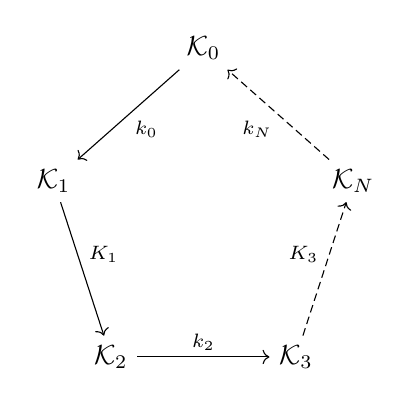
\begin{tikzpicture}[commutative diagrams/every diagram]
		\node (K0) at (90:2.3cm) {$\mathcal{K}_0$};
		\node (K1) at (90+72:2cm) {$\mathcal{K}_1$};
		\node (K2) at (90+2*72:2cm) {$\mathcal{K}_2$};
		\node (K3) at (90+3*72:2cm) {$\mathcal{K}_3$};
		\node (Kn) at (90+4*72:2cm) {$\mathcal{K}_N$};
		
		\path[commutative diagrams/.cd, every arrow, every label]
		(K0) edge node {$k_0$} (K1)
		(K1) edge node {$K_1$} (K2)
		(K2) edge node {$k_2$} (K3);
		
		\path[commutative diagrams/.cd, every arrow, every label, dashed]
		(K3) edge node {$K_3$} (Kn)
		(Kn) edge node {$k_N$} (K0);
\end{tikzpicture}
	\caption{The initial map.}
\end{figure}

A morphism in this category means that if the reflection functor on its start is executed just now, then the target functor will be executed next time. That is, to be more specific, if a functor in \(\mathcal{Q}\) has no morphisms targeting it, then it will be never executed unless it is configured as the beginning functor (location \(0\)) manually. Moreover, if a functor has more than one morphisms starting from it, then we call this functor \pmb{ extroverted}. Otherwise, if a functor has more than one morphisms targeting it, it is \pmb{ introverted}. If one has only two morphisms connected, one in and one out, thus it is\pmb{  ordinary}. The process of determining the next functor of a extroverted functor will be discussed below.

The definition below describes how the recursive functor uses the knowledge base and the further evolution for the data structure of the knowledge base. It ought to be paid attention to that although in the Introduction part that I say this new method of implementing a prover makes the prover low-knowledge and it turns out to have an infrastructure called the knowledge base. This is not conflictual since the knowledge I mean by in the Introduction section means the algorithm is automated, which means it does not require users to give in too much assistance and it does not know exactly what is under manipulation. On the other hand, however, the knowledge word here means by the storage of reflections, which can be rules, axioms, theorems, lemmas and even strategies.

\pmb{ Definition. }A recursive functor \(\mathcal{F}_i\) is a functor that applies to pool \(\mathcal{M}_i\) and evolves it into \(\mathcal{M}_{i+1}\). The process of determining which \(\mathcal{K}_w\) is \pmb{ selected} after former reflection functor \(\mathcal{K}_j\) generally works on the knowledge base \(\mathcal{Q}\), right starting from the initial map. If this is the first time for the recursive functor to execute, then \(\mathcal{K}_0\) is selected. If \(\mathcal{F}_i\) encounters with an introverted or ordinary functor \(\mathcal{K}_j\) then significantly,

\[w = k_j\left(\mathcal{K}_j\right)\]

If \(\mathcal{F}_i\) encounters with an extroverted functor, then the random number \(\mathit{r}\) is utilized and \(w\) turns out to be the following:

\[w = (\mathit{r} \bmod \sum _{u=0}^N )\left|\text{Hom}_{\mathcal{Q}}\left(\mathcal{K}_j,\mathcal{K}_q\right)\right|\]

It is easy to understand that for each reflection functor \(\mathcal{K}_a\) and \(\mathcal{K}_b\), the count of set \(\text{Hom}_{\mathcal{Q}}\left(\mathcal{K}_a,\mathcal{K}_b\right)\) indicates the \pmb{ weight} of \(\mathcal{K}_b\) to \(\mathcal{K}_a\), controlling the probability of \(\mathcal{K}_b\) to be selected when the former functor is \(\mathcal{K}_a\). The design of this process is inspired by the lottery scheduling algorithm I learned in Andrew S. Tanenbaum{'}s Operating Systems: Design and Implementation \cite{6} before.

An issue that worth attention is that as the random generator is defined as the following recursion formula: \cite{5}

\[X_{n+1}=(\left(1103515245 X_n+12345\right) \bmod 2^{32})\]

Then each \(\mathit{r}\) must belongs to region \(\mathbb{Z}_{\left.\left[0,2^{32}\right.\right)}\). That is, obviously, if \(\sum _{u=0}^N \left|\text{Hom}_{\mathcal{Q}}\left(\mathcal{K}_j,\mathcal{K}_q\right)\right|\geq 2^{32}\), then there will be some of the functors that will never be referred to, although there do exist morphisms targeting them. While in this paper the problem will not be solved and we assume that the number of the morphisms added up is smaller than the boundary of \(2^{32}\), which equals to four giga bytes and will not be exceeded in most engineering situations. Obviously although using the portable recursion equation the quality of the random numbers generated may be lower than nowadays{'} some technical implementations, it can be conveniently expressed in this paper. If the algorithm is implemented into the read world, a randomness collector, which generates random numbers from the real world, for example, the viberation of the computer motherboard, will probably act as a better solution.

It should be noted that if the initial map does not evolve, the proof efficiency will be primitive. Hence, we define a supplement process called \pmb{ knowledge reinforcement}, with definition coming below.

\pmb{ Definition.} The process of knowledge reinforcement is done after a finishing a proof. The first step of this reinforcement is to add numbers of utilization of the corresponding morphism of copies of morphisms into the knowledge base, increasing the weight of connections between the reflection functors. When next time a proof is issued, the modified knowledge base is \pmb{ loaded} into instance and act as the modified initial situation.

The second step of this sort of reinforcement is called \pmb{ reduction}, which is based on the Ebbinghaus{'}s forgetful curve{'}s numerical fit function. The exact form of the function expression can be found in the Preliminary section. Specifically, the number of morphisms is decreased following the forgetful equation, changing into the nearest integer number. To be more explicit, the Ebbinghaus-reduced decimal is stored separately from the knowledge base and the exact and accurate representation for this is omitted in the paper.

A situation after some reinforcements may be the one demonstrated in the figure below.

\begin{figure}[h]
	\centering
	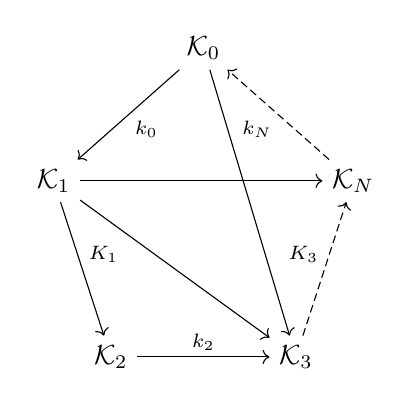
\begin{tikzpicture}[commutative diagrams/every diagram]
		\node (K0) at (90:2.3cm) {$\mathcal{K}_0$};
		\node (K1) at (90+72:2cm) {$\mathcal{K}_1$};
		\node (K2) at (90+2*72:2cm) {$\mathcal{K}_2$};
		\node (K3) at (90+3*72:2cm) {$\mathcal{K}_3$};
		\node (Kn) at (90+4*72:2cm) {$\mathcal{K}_N$};
		
		\path[commutative diagrams/.cd, every arrow, every label]
		(K0) edge node {$k_0$} (K1)
		(K1) edge node {$K_1$} (K2)
		(K2) edge node {$k_2$} (K3)
		(K1) edge node {} (K3)
		(K1) edge node {} (Kn)
		(K0) edge node {} (K3);
		
		\path[commutative diagrams/.cd, every arrow, every label, dashed]
		(K3) edge node {$K_3$} (Kn)
		(Kn) edge node {$k_N$} (K0);
	\end{tikzpicture}
	\caption{An example map after several reinforcements.}
\end{figure}

Via the process we described in the forth section and the data structures we presented in the third section, a mathematical proof can be conducted over category theory{'}s accurate representation. Then, a proof procedure is generated using the form of reflection history, that is, the historical list of the reflection functors utilized by the proof.

\section*{Conclusions and Future Work}

In the sections before I have presented an elegant data structure for representing mathematical concepts and a neat process which utilizes category theory concepts and knowledge to conduct proof, which also have self-optimization features.

Currently I have developed a computer program called DefQed that implements the algorithm and it is open-sourced with BSD 3-Clause {``}New{''} or {``}Revised{''} License on GitHub. The source code of the latest version can be accessed at \cite{7} It should be noted that the version is very early and some aspects of the algorithm I presented in the paper is not implemented.

Future works are the followings below:
\begin{itemize}
	\item \pmb{Continuing the implementation of the corresponding software.} Currently the software I developed is still under immature development and many of the aspects I presented in the paper above, including the self-evolution logic, have not been constructed yet.
	\item  \pmb{Improving the algorithm.} The algorithm I presented in the paper is not mature. For instance, if the knowledge base has more than \(2^{32}\) morphisms, then some of the morphisms will never be utilized.
	\item \pmb{Optimizing the performance of the algorithm.} Currently, though the design of the procedures increase generality because of the low-knowledge feature, the performance of derivations may be lower than the current algorithms, which focus on a certain subject inside mathematics.
\end{itemize}

\section*{Acknowledgments}
I express my sincerest greatest gratitude to my tutor Prof. Shao Xinhui, the Yingcai Project of P.R.China, which enables senior high school students to conduct science research, my senior high academy Northern Eastern Yucai School (NEYC) of P.R.China and the corresponding university Northern Eastern University (NEU) of P.R.China. I also thank my parents for encouraging me to conduct this research project.

\bibliographystyle{alpha}
\bibliography{document}
\end{document}